% !TEX encoding = UTF-8
% !TEX TS-program = pdflatex
% !TEX root = ../tesi.tex

%**************************************************************
\chapter{Analisi dei requisiti}
\label{ch:analisi-requisiti}
%**************************************************************

\intro{
In questa sezione viene presenta l'analisi dei requisiti, comprensivo dei casi d'uso, requisiti e il tracciamento di questi ultimi.
Per lo studio dei casi di utilizzo del prodotto sono stati creati dei diagrammi.
I diagrammi dei casi d'uso (in inglese \emph{Use Case Diagram}) sono diagrammi di tipo \gls{uml} dedicati alla descrizione delle funzioni o servizi offerti da un sistema, così come sono percepiti e utilizzati dagli attori che interagiscono col sistema stesso.
}\\


\section{Attori}\label{sec:attori}
L'unico utilizzatore del software \`{e} identificato come \textbf{attore generico} e ha il permesso di effettuare tutte le operazioni offerte dal tool.


\section{Casi d'uso}\label{sec:casi-d'uso}
\subsection*{UC-1 Selezione file}\label{subsec:uc-1-selezione-file}
\begin{itemize}
    \item \textbf{attori:} utente generico;
    \item \textbf{descrizione:} serve per permettere all'utente di selezionare il file APK da analizzare;
    \item \textbf{pre-condizioni:} l'utente ha avviato il tool;
    \item \textbf{post-condizioni:} l'utente ha selezionato un file di con estensione APK valido;
    \item \textbf{flusso degli eventi principali:}
    \begin{itemize}
        \item l'utente seleziona il file;
        \item l'utente conferma la selezione del file.
    \end{itemize}
\end{itemize}
\subsection*{UC-2 Avvio decompilazione}\label{subsec:uc-2-avvio-decompilazione}
\begin{itemize}
    \item \textbf{attori:} utente generico;
    \item \textbf{descrizione:} l'utente deve avviare la decompilazione del file APK;
    \item \textbf{pre-condizioni:} l'utente ha selezionato con successo un file APK;
    \item \textbf{post-condizioni:} la decompilazione è avvenuto con successo;
    \item \textbf{flusso degli eventi principali:}
    \begin{itemize}
        \item l'utente avvia la decompilazione;
        \item l'utente visualizza il messaggio della decompilazione avvenuto con successo;
    \end{itemize}
    \item \textbf{Estensione:}
    \begin{itemize}
        \item UC-3 Visualizzazione errore di decompilazione;
    \end{itemize}
\end{itemize}

\subsection*{UC-3 Visualizzazione errore di decompilazione}\label{subsec:uc-3-visualizzazione-errore-di-decompilazione}
\begin{itemize}
    \item \textbf{attori:} utente generico;
    \item \textbf{descrizione:} la decompilazione del file APK potrebbe generare degli errori;
    \item \textbf{pre-condizioni:} l'utente ha avviato la decompilazione dell'APK;
    \item \textbf{post-condizioni:} l'utente ha visualizzato il messaggio d'errore;
    \item \textbf{flusso degli eventi principali:}
    \begin{itemize}
        \item l'utente visualizza il messaggio di errore;
    \end{itemize}
\end{itemize}
\subsection*{UC-4 Installazione APK decompilato}\label{subsec:uc-4-installazione-apk-decompilato}
\begin{itemize}
    \item \textbf{attori:} utente generico;
    \item \textbf{descrizione:} permette all'utente d'installare l'apk, decompilato, manomesso e ricompilato, su un AVD;
    \item \textbf{pre-condizioni:} la decompilazione dell'APK è stato eseguito con successo;
    \item \textbf{post-condizioni:} l'APK è stato installato sull'AVD con successo;
    \item \textbf{flusso degli eventi principali:}
    \begin{itemize}
        \item l'utente seleziona un'AVD presente sul proprio computer;
        \item l'utente avvia l'installazione dell'APK ricompilato;
        \item l'utente visualizza un messaggio d'installazione avvenuto con successo;
    \end{itemize}
\end{itemize}
\subsubsection*{UC-4.1 Selezione AVD}\label{subsubsec:uc-4.1-selezione-avd}
\begin{itemize}
    \item \textbf{attori:} utente generico;
    \item \textbf{descrizione:} serve per permettere all'utente di selezionare un'AVD presente nel proprio computer;
    \item \textbf{pre-condizioni:} l'utente ha avviato il software;
    \item \textbf{post-condizioni:} l'utente ha selezionato l'AVD da avviare;
    \item \textbf{flusso degli eventi principali:}
    \begin{itemize}
        \item l'utente visualizza un elenco delle AVD presenti nel proprio computer;
        \item l'utente seleziona un'AVD;
        \item l'utente conferma la selezione;
        \item l'AVD selezionato si è avviato con successo
    \end{itemize}
    \item \textbf{Estensione}
    \begin{itemize}
        \item UC-5 Visualizzazione messaggio nessun AVD rilevato;
    \end{itemize}
\end{itemize}
\begin{figure}
    \centering
    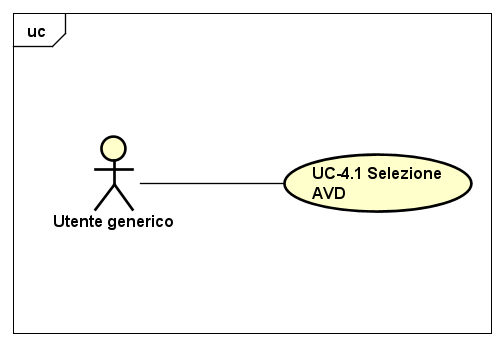
\includegraphics[width=10cm, height=8cm]{./usecase/uc_4_1.png}
    \caption{Sottocaso d'uso UC-4.1 Selezione AVD}
\end{figure}

\subsection*{UC-5 Visualizzazione messaggio nessun AVD rilevato} \label{subsec:uc-5-visualizzazione-messaggio-nessun-avd-rilevato}
\begin{itemize}
    \item \textbf{attori:} utente generico;
    \item \textbf{descrizione:} quando non sono presenti nessun AVD o il tool non è riuscito a rilevarne, viene mostrato un messaggio all'utente;
    \item \textbf{pre-condizioni:} l'utente ha aperto il tool;
    \item \textbf{post-condizioni:} l'utente ha visualizzato il messaggio;
    \item \textbf{flusso degli eventi principali:}
    \begin{itemize}
        \item l'utente visualizza il messaggio;
    \end{itemize}
\end{itemize}
\subsection*{UC-6 Errore durante avvio dell'AVD}\label{subsec:uc-6-errore-durante-avvio-dell'avd}
\begin{itemize}
    \item \textbf{attori:} utente generico;
    \item \textbf{descrizione:} serve a mostrare all'utente gli eventuali errori durante l'avvio dell'AVD;
    \item \textbf{pre-condizioni:} l'utente ha selezionato un'AVD e ha confermato l'avvio;
    \item \textbf{post-condizioni:} l'utente ha visualizzato il messaggio d'errore;
    \item \textbf{flusso degli eventi principali:}
    \begin{itemize}
        \item l'utente visualizza il messaggio d'errore;
    \end{itemize}
\end{itemize}
\subsection*{UC-7 Dump dello storage interno}\label{subsec:uc-6-dump-dello-storage-interno}
\begin{itemize}
    \item \textbf{attori:} utente generico;
    \item \textbf{descrizione:} nel caso l'utente volesse una copia dei dati interni dell'applicativo, ha bisogno di fare il dump;
    \item \textbf{pre-condizioni:} l'installazione dell'APK manomesso è andato a buon fine;
    \item \textbf{post-condizioni:} è stato fatto una copia dello storage interno;
    \item \textbf{flusso degli eventi principali:}
    \begin{itemize}
        \item l'utente seleziona la voce "copia i dati interni";
        \item l'utente seleziona il path dove collocare i dati;
    \end{itemize}
\end{itemize}
\subsection*{UC-8 Decodifica del codice}\label{subsec:uc-8-decodifica-del-codice}
\begin{itemize}
    \item \textbf{attori:} utente generico;
    \item \textbf{descrizione:} durante la decompilazione dell'APK vengono creati dei file .dex che contengono il codice sorgente dell'APK, e questo caso d'uso serve per permettere all'utente di ottenere il codice sorgente;
    \item \textbf{pre-condizioni:} la decompilazione è avvenuto con successo;
    \item \textbf{post-condizioni:} l'utente ha ottenuto una copia del codice sorgente in java;
    \item \textbf{flusso degli eventi principali:}
    \begin{itemize}
        \item l'utente ha selezionato la funzionalità decodifica dei dex;
        \item l'utente seleziona il percorso dove posizionare il codice sorgente ottenuto;
        \item l'utente ha salvato il codice sorgente ottenuto.
    \end{itemize}
\end{itemize}
\subsubsection*{UC-8.1 Avvio decodifica}
\begin{itemize}
    \item \textbf{attori:} utente generico;
    \item \textbf{descrizione:} serve all'utente per avviare la decodifica dei file .dex;
    \item \textbf{pre-condizioni:} la decompilazione dell'APK è avvenuto correttamente;
    \item \textbf{post-condizioni:} la decodifica è avvenuto con successo;
    \item \textbf{flusso degli eventi principali:}
    \begin{itemize}
        \item l'utente seleziona la funzionalità di decodifica dei file .dex;
    \end{itemize}
\end{itemize}
\subsubsection*{UC-8.2 Salvataggio del codice decodificato}
\begin{itemize}
    \item \textbf{attori:} utente generico;
    \item \textbf{descrizione:} serve all'utente per salvare i codici sorgenti decodificati;
    \item \textbf{pre-condizioni:} la decompilazione è avvenuto con successo;
    \item \textbf{post-condizioni:} i file con i codici sorgenti sono stati salvati correttamente;
    \item \textbf{flusso degli eventi principali:}
    \begin{itemize}
        \item l'utente seleziona la voce "salva file decodificati";
        \item l'utente seleziona la posizione dove vuole salvare i file;
        \item i file vengono salvati correttamente.
    \end{itemize}
\end{itemize}

\begin{figure}[H]
    \centering
    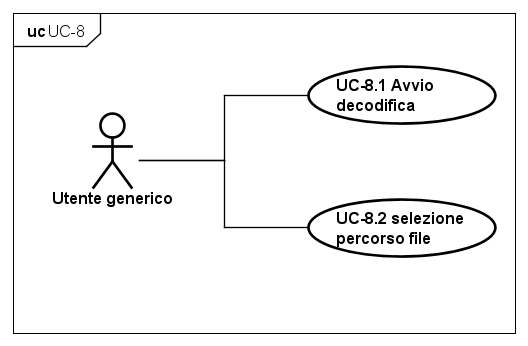
\includegraphics[width=10cm, height=8cm]{./immagini/usecase/uc_8.png}
    \caption{Caso d'uso UC-8 Decodifica codici .dex}
\end{figure}



\subsection*{UC-9 Visualizzazione errore decodifica}\label{subsec:uc-9-visualizzazione-errore-decodifica}
\begin{itemize}
    \item \textbf{attori:} utente generico;
    \item \textbf{descrizione:} durante la decodifica dei .dex possono sorgere molteplici errori;
    \item \textbf{pre-condizioni:} l'utente ha selezionato la funzionalità di decodifica del codice .dex;
    \item \textbf{post-condizioni:} l'utente ha visualizzato il messaggio di errore durante la decodifica;
    \item \textbf{flusso degli eventi principali:}
    \begin{itemize}
        \item l'utente ha visualizzato il messaggio d'errore;
    \end{itemize}
\end{itemize}

\begin{figure}[H]
    \centering
    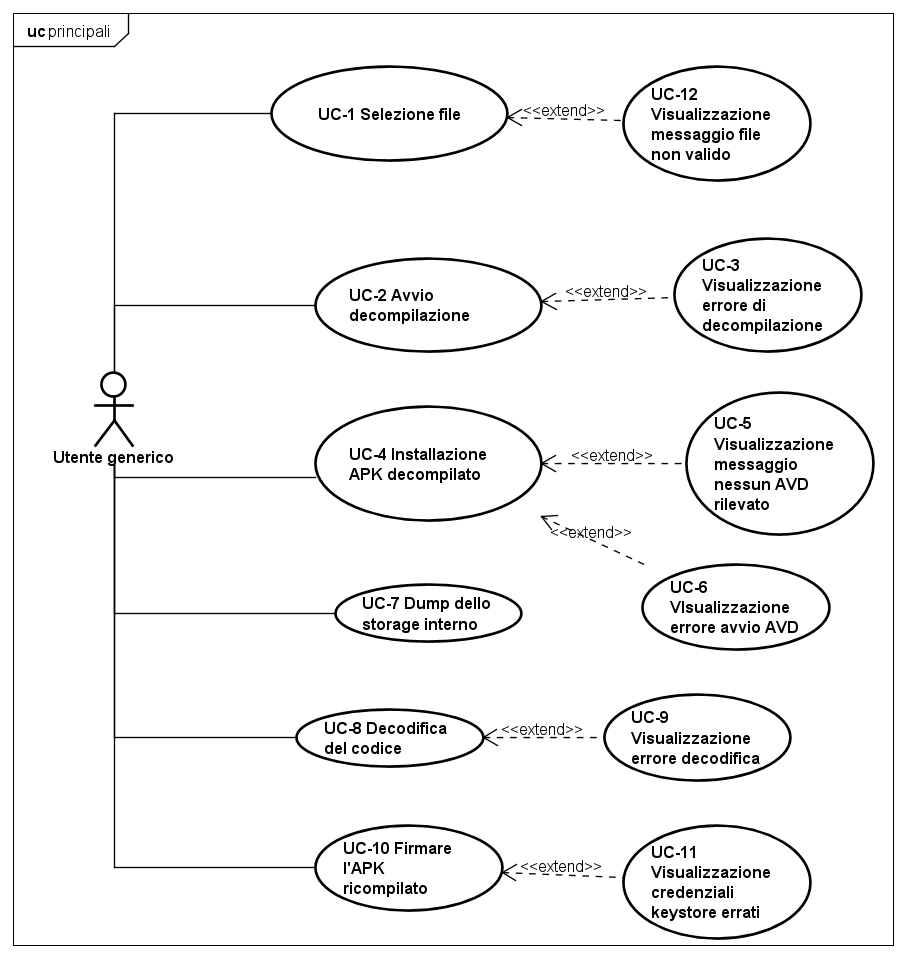
\includegraphics[width=10cm, height=8cm]{./immagini/usecase/uc_principali.png}
    \caption{Casi d'uso da 1 a 12}
\end{figure}

\subsection*{UC-10 Firmare l'APK ricompilato}\label{subsec:uc-10-firmare-l'apk-ricompilato}
\begin{itemize}
    \item \textbf{attori:} utente generico;
    \item \textbf{descrizione:} dopo la ricompilazione si può firmare l'APK;
    \item \textbf{pre-condizioni:} la ricompilazione dell'APK è avvenuto correttamente;
    \item \textbf{post-condizioni:} l'APK è stata firmata correttamente;
    \item \textbf{flusso degli eventi principali:}
    \begin{itemize}
        \item UC-10.1 selezione keystore;
        \item UC-10.3 inserimento alias;
        \item UC-10.4 inserimento password.
    \end{itemize}
    \item \textbf{Estensione}
    \begin{itemize}
        \item UC-11 Visualizzazione credenziali keystore errati;
    \end{itemize}
\end{itemize}
\subsubsection*{UC-10.1 Selezione keystore}\label{subsubsec:uc-10.1-selezione-keystore}
\begin{itemize}
    \item \textbf{attori:} utente generico;
    \item \textbf{descrizione:} permettere all'utente di selezionare il keystore da utilizzare per firmare l'APK;
    \item \textbf{pre-condizioni:} la ricompilazione dell'APK è avvenuto correttamente;
    \item \textbf{post-condizioni:} è stato selezionato un file di tipo keystore corretto (estensione: \textbf{.jks});
    \item \textbf{flusso degli eventi principali:}
    \begin{itemize}
        \item l'utente seleziona la funzionalità per selezionare il keystore;
        \item l'utente seleziona il keystore;
    \end{itemize}
    \item \textbf{flussi secondari}
    \begin{itemize}
        \item UC-10.2 Visualizzazione messaggio file selezionato non valido;
    \end{itemize}
\end{itemize}
\subsubsection*{UC-10.2 Visualizzazione messaggio file selezionato non valido}
\begin{itemize}
    \item \textbf{attori:} utente generico;
    \item \textbf{descrizione:} l'utente, al quale è stato chiesto di selezionare un file di tipo keystore, potrebbe selezionare un file non valido;
    \item \textbf{pre-condizioni:} l'utente ha selezionato un file;
    \item \textbf{post-condizioni:} il messaggio di errore è stato mostrato;
    \item \textbf{flusso degli eventi principali:}
    \begin{itemize}
        \item l'utente visualizza il messaggio d'errore.
    \end{itemize}
\end{itemize}
\subsubsection*{UC-10.3 Inserimento Alias}
\begin{itemize}
    \item \textbf{attori:} utente generico;
    \item \textbf{descrizione:} l'utente deve inserire l'alias della chiave da utilizzare durante la firma dell'APK;
    \item \textbf{pre-condizioni:} l'utente ha selezionato un keystore valido;
    \item \textbf{post-condizioni:} l'utente ha inserito l'alias da utilizzare;
    \item \textbf{flusso degli eventi principali:}
    \begin{itemize}
        \item l'utente inserisce l'alias della chiave da utilizzare per firmare l'APK;
    \end{itemize}
\end{itemize}
\subsubsection*{UC-10.4 Inserimento password}
\begin{itemize}
    \item \textbf{attori:} utente generico;
    \item \textbf{descrizione:} l'utente deve inserire la password del keystore da utilizzare durante la firma dell'APK;
    \item \textbf{pre-condizioni:} l'utente ha selezionato un keystore valido;
    \item \textbf{post-condizioni:} l'utente ha inserito la password da utilizzare;
    \item \textbf{flusso degli eventi principali:}
    \begin{itemize}
        \item l'utente inserisce la password;
    \end{itemize}
\end{itemize}
\begin{figure}[H]
    \centering
    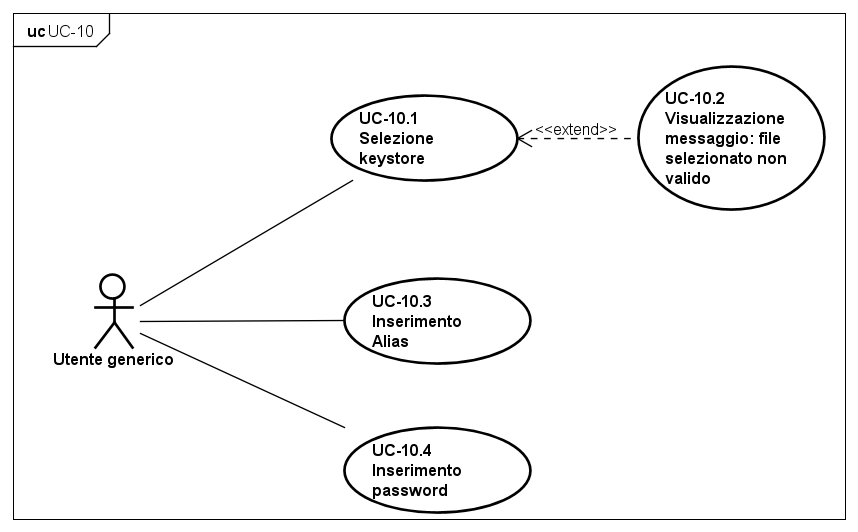
\includegraphics[width=10cm, height=8cm]{./immagini/usecase/uc_10.png}
    \caption{Sottocasi d'uso del caso d'uso UC-10}
\end{figure}

\subsection*{UC-11 Visualizzazione credenziali keystore errati}\label{subsec:uc-11-visualizzazione-credenziali-keystore-errati}
\begin{itemize}
    \item \textbf{attori:} utente generico;
    \item \textbf{descrizione:} per firmare l'APK l'utente deve inserire dei credenziali, e quando quest'ultimi sono errati viene mostrato un messaggio di errore;
    \item \textbf{pre-condizioni:} l'utente ha selezionato la funzionalità per ricompilare l'APK;
    \item \textbf{post-condizioni:} l'utente ha visualizzato il messaggio di errore;
    \item \textbf{flusso degli eventi principali:}
    \begin{itemize}
        \item l'utente ha visualizzato l'errore;
    \end{itemize}
\end{itemize}

\subsection*{UC-12 Visualizzazione messaggio file non valido}\label{subsec:uc-12-visualizzazione-messaggio-file-non-valido}
\begin{itemize}
    \item \textbf{attori:} utente generico;
    \item \textbf{descrizione:} quando l'utente seleziona un file che non ha l'estensione APK un messaggio deve essere mostrato all'utente;
    \item \textbf{pre-condizioni:} l'utente ha selezionato un file non APK;
    \item \textbf{post-condizioni:} l'utente ha visualizzato il messaggio d'errore;
    \item \textbf{flusso degli eventi principali:}
    \begin{itemize}
        \item l'utente visualizza il messaggio d'errore.
    \end{itemize}
\end{itemize}
\subsection*{UC-13 Decodifica dei file \textit{.dex} in file \textit{.java}}\label{subsec:uc-13-decodifica-dei-filetextitin-filetextit}
\begin{itemize}
    \item \textbf{attori:} utente generico;
    \item \textbf{descrizione:} dall'APK ricompilato si ottengono dei file \textit{.dex} che possono essere convertiti in \textit{.class} e quindi in \textit{.java};
    \item \textbf{pre-condizioni:} la decompilazione dell'APK \`{e} andata a buon fine;
    \item \textbf{post-condizioni:} la decodifica dei file \textit{.dex} in \textit{.java} \`{e} andata a buon fine;
    \item \textbf{flusso degli eventi principali:}
    \begin{itemize}
        \item l'utente seleziona la voce "Decodifica Dex".
    \end{itemize}
\end{itemize}

\subsection*{UC-14 Analisi del codice \textit{.java}}\label{subsec:uc-14-analisi-del-codicetextit}
\begin{itemize}
    \item \textbf{attori:} attore generico;
    \item \textbf{descrizione:} dopo aver ottenuto i file \textit{.java} eseguendo il caso d'uso UC-13, si potr\`{a} effettuare dell'analisi sul codice;
    \item \textbf{pre-condizioni:} la decodifica dei file \textit{.dex} in \textit{.java} \`{e} andata a buon fine;
    \item \textbf{post-condizioni:} viene generato un pdf con i risultati dell'analisi;
    \item \textbf{flusso degli eventi principali:}
    \begin{itemize}
        \item l'utente seleziona la voce "analyze";
        \item l'utente seleziona le opzioni di analisi;
        \item all'analisi completato, l'utente specifica dove posizionare il file pdf con i risultati dell'analisi;
        \item il file viene salvato nel percorso da lui specificato.
    \end{itemize}
\end{itemize}
\begin{figure}[H]
    \centering
    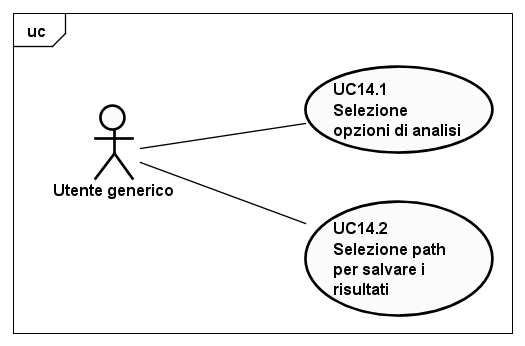
\includegraphics[width=10cm, height=8cm]{./immagini/usecase/uc_14_1_14_2.png}
    \caption{Sottocasi d'uso del caso d'uso 14}
\end{figure}



\subsection*{UC-15 avvio AVD}\label{subsec:uc-15-avvio-avd}
\begin{itemize}
    \item \textbf{attori:} attore generico;
    \item \textbf{descrizione:} serve per avviare un'avd per poter eseguire l'applicazione;
    \item \textbf{pre-condizioni:} il tool è stato avviato correttamente e nel sistema è presente almeno un AVD;
    \item \textbf{post-condizioni:} l'AVD è stato avviato correttamente;
    \item \textbf{flusso degli eventi principali:}
    \begin{itemize}
        \item l'attore visualizza l'elenco delle AVD presenti nel sistema;
        \item l'attore seleziona un'AVD che vuole avviare;
        \item l'attore seleziona se utilizzare un proxy da impostare nell'AVD;
        \item l'attore seleziona la voce avvia AVD.
    \end{itemize}
    \item \textbf{estensione:} UC-5 Visualizzazione messaggio nessun AVD rilevato.
\end{itemize}
\subsection*{UC-16 avvio AVD senza proxy}\label{subsec:uc-16-avvio-avd-senza-proxy}
\begin{itemize}
    \item \textbf{attori:} attore generico;
    \item \textbf{descrizione:} quando l'attore decide che non vuole avviare l'AVD modificando le impostazioni di proxy, viene eseguito questo caso d'uso;
    \item \textbf{pre-condizioni:} l'attore ha avviato correttamente il tool e nel sistema è presente almeno un'AVD;
    \item \textbf{post-condizioni:} l'AVD è stato avviato correttamente con le impostazioni di proxy di default;
    \item \textbf{flusso degli eventi principali:}
    \begin{itemize}
        \item l'attore visualizza l'elenco delle AVD presenti nel sistema;
        \item l'attore seleziona un'AVD che vuole avviare;
        \item l'attore seleziona di non utilizzare un proxy da impostare nell'AVD;
        \item l'attore seleziona la voce avvia AVD.
    \end{itemize}
\end{itemize}
\subsection*{UC-17 avvio AVD con proxy}\label{subsec:uc-16-avvio-avd-con-proxy}
\begin{itemize}
    \item \textbf{attori:} attore generico;
    \item \textbf{descrizione:} quando l'attore decide che non vuole avviare l'AVD modificando le impostazioni di proxy, viene eseguito questo caso d'uso;
    \item \textbf{pre-condizioni:} l'attore ha avviato correttamente il tool e nel sistema è presente almeno un'AVD;
    \item \textbf{post-condizioni:} l'AVD è stato avviato correttamente con le impostazioni di proxy inseriti;
    \item \textbf{flusso degli eventi principali:}
    \begin{itemize}
        \item l'attore visualizza l'elenco delle AVD presenti nel sistema;
        \item l'attore seleziona un'AVD che vuole avviare;
        \item l'attore seleziona di utilizzare un proxy da impostare nell'AVD;
        \item l'attore inserisce le informazioni del proxy, per esempio: \textit{localhost:8080};
        \item l'attore seleziona la voce avvia AVD.
    \end{itemize}
\end{itemize}
\subsubsection*{UC-17.1 Selezione voce Avvia con proxy}
\begin{itemize}
    \item \textbf{attori:} attore generico;
    \item \textbf{descrizione:} l'utente vuole avviare l'AVD con le opzioni di proxy;
    \item \textbf{pre-condizioni:} il tool è stato avviato correttamente ed è riuscito a rilevare gli AVD presenti nel sistema;
    \item \textbf{post-condizioni:} l'opzione di proxy è stato selezionato;
    \item \textbf{flusso degli eventi principali:}
    \begin{itemize}
        \item l'utente seleziona la voce per avviare l'AVD.
    \end{itemize}
\end{itemize}
\subsubsection*{UC-17.2 selezione voce avvio AVD}
\begin{itemize}
    \item \textbf{attori:} attore generico;
    \item \textbf{descrizione:} l'utente avviare l'AVD;
    \item \textbf{pre-condizioni:} l'utente ha selezionato le opzioni per avviare l'AVD;
    \item \textbf{post-condizioni:} il tool avvia l'AVD;
    \item \textbf{flusso degli eventi principali:}
    \begin{itemize}
        \item il tool seleziona la voce avvio di avviare l'AVD.
    \end{itemize}
\end{itemize}
\subsubsection*{UC-17.3 inserimento indirizzo e porta proxy}
\begin{itemize}
    \item \textbf{attori:} attore generico;
    \item \textbf{descrizione:} serve all'attore per inserire i dati del proxy;
    \item \textbf{pre-condizioni:} l'utente ha selezionato l'opzione di avviare l'AVD con il proxy;
    \item \textbf{post-condizioni:} i dati sono stati inseriti correttamente;
    \item \textbf{flusso degli eventi principali:}
    \begin{itemize}
        \item l'utente inserisce l'indirizzo IP del server proxy;
        \item l'utente inserisce il numero della porta del server proxy.
    \end{itemize}
\end{itemize}
\subsubsection*{UC-17.4 conferma dei dati}
\begin{itemize}
    \item \textbf{attori:} attore generico;
    \item \textbf{descrizione:} serve all'utente per confermare i dati inseriti per avviare l'AVD;
    \item \textbf{pre-condizioni:} l'utente ha inserito le opzioni di proxy correttamente;
    \item \textbf{post-condizioni:} l'AVD è stato avviato correttamente con le opzioni di proxy;
    \item \textbf{flusso degli eventi principali:}
    \begin{itemize}
        \item l'utente conferma le informazioni inserite e avvia l'AVD.
    \end{itemize}
\end{itemize}

\begin{figure}[H]
    \centering
    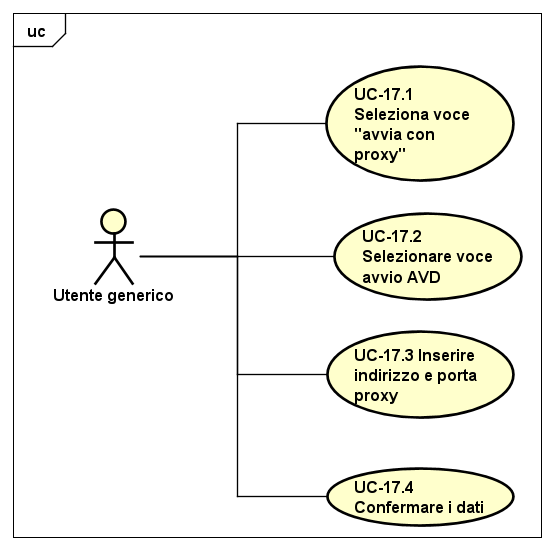
\includegraphics[width=10cm, height=8cm]{./immagini/usecase/uc_17.png}
    \caption{Sottocasi d'uso del caso d'uso 17}
\end{figure}
\subsection*{UC-18 Inizio registrazione traffico di rete}\label{subsec:uc-18-inizio-registrazione-traffico-di-rete}
\begin{itemize}
    \item \textbf{attori:} attore generico;
    \item \textbf{descrizione:} quando l'utente vuole registrare le attività di rete effettuate dall'AVD eseguendo l'applicazione, può utilizzare questa funzionalità;
    \item \textbf{pre-condizioni:} l'attore ha avviato l'applicazione;
    \item \textbf{post-condizioni:} l'attore ha registrato le attività di rete e ottenuto un file cap;
    \item \textbf{flusso degli eventi principali:}
    \begin{itemize}
        \item l'attore seleziona la voce "Start record!";
        \item l'attore successivamente seleziona la voce "Stop Record".
    \end{itemize}
\end{itemize}
\begin{figure}[H]
    \centering
    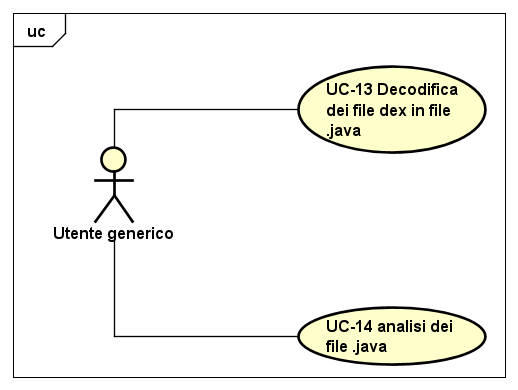
\includegraphics[width=10cm, height=8cm]{./immagini/usecase/UC-13_14.png}
    \caption{Casi d'uso da 13 a 18}
\end{figure}

%\subsection*{UC-}
%\begin{itemize}
%    \item \textbf{attori:} attore generico;
%    \item \textbf{descrizione:}
%    \item \textbf{pre-condizioni:}
%    \item \textbf{post-condizioni:}
%    \item \textbf{flusso degli eventi principali:}
%    \begin{itemize}
%    \end{itemize}
%\end{itemize}
\section{Tracciamento dei requisiti}\label{sec:tracciamento-dei-requisiti}
\newcounter{rowcount}
\setcounter{rowcount}{0}
\newcounter{subCount}
\setcounter{subCount}{0}

\subsection{Classificazione}\label{subsec:classificazione}
Di seguito sono riportati i requisiti individuati durante l'attività di analisi.
Tali requisiti sono stati individuati dai casi d'uso, dal piano di lavoro e dai colloqui con il tutor aziendale \tutorAziendale.
I requisiti individuati sono stati divisi in:
\begin{itemize}
    \item \textbf{Requisiti funzionali:} insieme di requisiti che definiscono le azioni fondamentali che devono avvenire in grado di processare un input e di generare un output;
    \item \textbf{Requisiti dichiarativi:} insieme di requisiti che rappresentano un vincolo di natura realizzativa, normativa o contrattuale;
    \item \textbf{Requisiti qualitativi:} insieme di requisiti che garantiscono una certa qualità al prodotto e che indicano le best practice usate per la realizzazione.
\end{itemize}
Inoltre, a ogni requisito è stata assegnata un'importanza:
\begin{itemize}
    \item \textbf{Obbligatori:} requisito al quale non si può rinunciare, indispensabile per il corretto funzionamento del prodotto;
    \item \textbf{Desiderabile:} requisito non necessario ma che porta valore aggiunto al prodotto;
    \item \textbf{Facoltativo:} requisito che risulta essere relativamente utile oppure contrattabile con il proponente in un momento successivo.
\end{itemize}

\subsection{Requisiti funzionali}\label{subsec:requisiti-funzionali}
Di seguiti sono elencati i requisiti derivanti dai casi d'uso individuati dalla sezione precedente.
\begin{longtable}{ | c| C{7cm} |C{3cm} |}
    \hline
    \textbf{Identificativo} & \textbf{Descrizione}                                                                                                  & \textbf{Fonte} \\\hline
    \idRequisiti{F-O}       & Il tool deve permettere di selezionare un file APK.                                                                   & UC-1           \\\hline
    \idRequisitiSub{F-O}    & Il tool deve permettere di mostrare un messaggio di errore se file selezionato non è valido.                          & UC-1           \\\hline
    \setcounter{subCount}{0}

    \idRequisiti{F-O}       & Il tool deve permettere di avviare la decompilazione dell'APK selezionato.                                            & UC-2           \\\hline
    \idRequisitiSub{F-O}    & Il tool deve permettere di visualizzare un messaggio di decompilazione avvenuto con successo.                         & UC-2           \\\hline
    \idRequisitiSub{F-O}    & Il tool deve aggiungere il flag android:debuggable="true" nel AndroidManifest.xml del decompilato.                    & UC-2           \\\hline
    \setcounter{subCount}{0}

    \idRequisiti{F-O}       & Il tool deve permettere di visualizzare il messaggio di errore quando la decompilazione non è terminato con successo. & UC-3           \\\hline
    \idRequisiti{F-O}       & Il tool deve permettere d'installare l'APK decompilato e modificato su un AVD.                                         & UC-4           \\\hline
    \idRequisitiSub{F-D}    & Il tool deve permettere di ricompilare l'APK decompilato.                                                             & UC-4           \\\hline
    \idRequisitiSub{F-D}    & Il tool deve permettere di avviare l'applicazione.                                                                    & UC-4           \\\hline
%        \setcounter{subCount}{0}

    \idRequisitiSub{F-O}    & Il tool deve permettere di selezionare un'AVD presente nel sistema.                                                   & UC-4           \\\hline
    \idRequisitiSub{F-O}    & Il tool deve permettere di visualizzare l'elenco delle AVD presenti nel sistema operativo.                            & UC-4           \\\hline
    \idRequisitiSub{F-O}    & Il tool deve permettere di confermare la selezione dell'AVD.                                                          & UC-4           \\\hline
    \setcounter{subCount}{0}

    \idRequisiti{F-O}       & Il tool deve permettere di visualizzare il messaggio quando non sono stati rilevati nessun AVD.                       & UC-5           \\\hline
    \idRequisiti{F-O}       & Il tool deve permettere di visualizzare il messaggio di errore se l'AVD selezionato non si è avviato correttamente.   & UC-6           \\\hline
    \idRequisiti{F-O}       & Il tool deve permettere di fare il dump dello storage interna dell'applicazione.                                      & UC-7           \\\hline
    \idRequisitiSub{F-O}    & Il tool deve permettere di selezionare il path dove collocare i dati copiati.                                         & UC-7           \\\hline
    \setcounter{subCount}{0}

    \idRequisiti{F-D}       & Il tool deve permettere di visualizzare i dex ottenuti dalla decompilazione.                                          & UC-8           \\\hline
    \idRequisitiSub{F-O}    & Il tool deve permettere di visualizzare il messaggio quando la decodifica è avvenuta con successo.                    & UC-8           \\\hline
    \idRequisitiSub{F-O}    & Il tool deve permettere di far selezionare il dex che l'utente vuole decodificare.                                    & UC-8           \\\hline
    \idRequisitiSub{F-O}    & Il tool deve permettere di confermare la selezione del dex da decodificare.                                           & UC-8           \\\hline
    \idRequisitiSub{F-O}    & Il tool deve permettere di far selezionare il path di dove salvare i file ottenuti dalla decodifica.                  & UC-8           \\\hline
    \setcounter{subCount}{0}

    \idRequisiti{F-O}       & Il tool deve permettere di visualizzare il messaggio d'errore se la decodifica non è andato a buon fine.              & UC-9           \\\hline

    \idRequisiti{F-F}       & Il tool deve permettere di firmare l'APK ricompilato.                                                                 & UC-10          \\\hline
    \idRequisitiSub{F-F}    & Il tool deve permettere di selezionare un file di tipo keystore.                                                      & UC-10          \\\hline
    \idRequisitiSub{F-F}    & Il tool deve permettere di mostrare un messaggio di errore quando viene selezionato un file non keystore.             & UC-10          \\\hline
    \idRequisitiSub{F-F}    & Il tool deve permettere d'inserire l'alias della chiave da utilizzare.                                                & UC-10          \\\hline
    \idRequisitiSub{F-F}    & Il tool deve permettere d'inserire la password del keystore da utilizzare.                                            & UC-10          \\\hline
    \setcounter{subCount}{0}

    \idRequisiti{F-F}       & Il tool deve permettere di mostrare dei messaggi quando le credenziali inseriti non sono corretti.                    & UC-11          \\\hline
    \idRequisiti{F-O}       & Il tool deve permettere di mostrare dei messaggi quando è stato selezionato un file non valido.                       & UC-12          \\\hline
    \idRequisiti{F-O}       & Il tool deve permettere di decodificare i file \textit{.dex} in \textit{.java}                                        & UC-13          \\\hline
    \idRequisiti{F-O}       & Il tool deve permettere di permettere di effettuare dell'analisi del codice java                                      & UC-14          \\\hline
    \idRequisitiSub{F-O}    & Il tool deve permettere di selezionare diverse opzioni di analisi                                                     & UC-14.1        \\\hline
    \idRequisitiSub{F-O}    & Il tool deve permettere di selezionare il path dove collocare i risultati dell'analisi.                               & UC-14.2        \\\hline
    \setcounter{subCount}{0}

    \idRequisiti{F-D}       & Il tool deve permettere di avviare un'AVD presente nel sistema.                                                       & UC-15          \\\hline
    \idRequisitiSub{F-D}    & Il tool deve permettere di visualizzare l'elenco delle AVD presenti nel sistema operativo.                            & UC-15          \\\hline
    \idRequisitiSub{F-D}    & Il tool deve permettere di selezionare un'AVD presente nel sistema.                                                   & UC-15          \\\hline
    \idRequisitiSub{F-D}    & Il tool deve permettere di specificare se avviare l'AVD con opzione di proxy.                                         & UC-15          \\\hline
    \setcounter{subCount}{0}
    \idRequisiti{F-D}       & Il tool deve permettere d'inserire le informazioni per il proxy.                                                      & UC-17          \\\hline
    \idRequisitiSub{F-D}    & Il tool deve permettere d'inserire l'indirizzo del server proxy.                                                      & UC-17          \\\hline
    \idRequisitiSub{F-D}    & Il tool deve permettere d'inserire il numero di porta del server proxy.                                               & UC-17          \\\hline
    \setcounter{subCount}{0}
    \idRequisiti{F-D}       & Il tool deve permettere di registrare il traffico di rete.                                                            & UC-18          \\\hline
    \idRequisitiSub{F-D}    & Il tool deve generare il file che contiene i dettagli del traffico di rete.                                           & UC-18          \\\hline
    \caption{Requisiti funzionali}
\end{longtable}

\setcounter{rowcount}{0}

\subsection{Requisiti di vincolo}\label{subsec:requisiti-vincolo}
\begin{center}
    \begin{longtable}{ | c| C{7cm} |C{3cm} |}
        \hline
        \textbf{Identificativo} & \textbf{Descrizione}                                              & \textbf{Fonte}   \\\hline
        \idRequisiti{V-D}       & Il tool può essere un tool da righe di comando                   & Piano di lavoro. \\\hline
        \idRequisiti{V-D}       & Il tool può essere un tool dotato di GUI                          & Piano di lavoro. \\\hline
        \idRequisiti{V-D}       & Il tool può essere sviluppato in JAVA                             & Piano di lavoro. \\\hline
        \idRequisiti{V-F}       & Il tool può essere sviluppato utilizzando i linguaggi funzionali. & Piano di lavoro. \\\hline
        \caption{Requisiti di vincolo}
    \end{longtable}
\end{center}
\setcounter{rowcount}{0}

\subsection{Requisiti qualitativi}\label{subsec:requisiti-qualitativi}
\begin{center}
    \begin{longtable}{ | c| C{7cm} |C{3cm} |}
        \hline
        \textbf{Identificativo} & \textbf{Descrizione}                                                                           & \textbf{Fonte}  \\\hline
        \idRequisiti{Q-O}       & Il codice sorgente deve essere versionato col sistema di versionamento dell'azienda ospitante. & Piano di lavoro \\\hline
        \idRequisiti{Q-O}       & Il Il codice sorgente deve essere sotto licenza GPL v3.                                        & Piano di lavoro \\\hline
%        \idRequisiti{Q-O}&Il code coverage dei test unitari deve superare 80\%.& Piano di lavoro\\\hline
%        \idRequisiti{Q-D}&Il code coverage dei test unitari deve essere 100\%.& Piano di lavoro\\\hline
        \caption{Requisiti qualitativi}
    \end{longtable}
\end{center}
\setcounter{subCount}{0}
\setcounter{rowcount}{0}
\section{Tracciamento fonte - requisiti}\label{sec:tracciamento-fonte---requisiti}

\begin{center}
    \begin{longtable}{| C{6cm} |C{6cm}|}
        \hline
        \textbf{Fonte} & \textbf{Requisito} \\\hline
        UC-1 &
        \begin{itemize}\itemsep0em
            \item R-1-F-O
            \item R-1.1-F-O
        \end{itemize}
        \\\hline
        UC-2 &
        \begin{itemize}\itemsep0em
            \item R-2-F-O
            \item R-2.1-F-O
            \item R-2.2-F-O
        \end{itemize}
        \\\hline
        UC-3 &
        \begin{itemize}\itemsep0em
            \item R-3-F-O
        \end{itemize} \\\hline
        UC-4 &
        \begin{itemize}\itemsep0em
            \item R-4-F-O
            \item R-4.1-F-D
            \item R-4.2-F-D
            \item R-4.3-F-O
            \item R-4.4-F-O
            \item R-4.5-F-O
            \item R-4.6-F-O
        \end{itemize} \\\hline
        UC-5 &
        \begin{itemize}\itemsep0em
            \item R-6-F-O
        \end{itemize} \\\hline
        UC-6 &
        \begin{itemize}\itemsep0em
            \item R-7-F-O
        \end{itemize} \\\hline
        UC-7 &
        \begin{itemize}\itemsep0em
            \item R-8-F-O
            \item R-8.1-F-O
        \end{itemize} \\\hline
        UC-8 &
        \begin{itemize}\itemsep0em
            \item R-9-F-D
            \item R-9.1-F-O
            \item R-9.2-F-O
            \item R-9.3-F-O
        \end{itemize} \\\hline
        UC-8.2 &
        \begin{itemize}\itemsep0em
            \item R-9.4-F-O
        \end{itemize} \\\hline
        UC-9 & \begin{itemize}\itemsep0em
                   \item R-10-F-O
        \end{itemize} \\\hline
        UC-10 &
        \begin{itemize}\itemsep0em
            \item R-11-F-F
            \item R-11.1-F-F
            \item R-11.2-F-F
            \item R-11.3-F-F
            \item R-11.4-F-F
            \item R-11.4-F-F
        \end{itemize}
        \\\hline

        UC-11 &
        \begin{itemize}\itemsep0em
            \item R-12-F-F
        \end{itemize}
        \\\hline

        UC-12 &
        \begin{itemize}\itemsep0em
            \item R-13-F-O
        \end{itemize}
        \\\hline

        UC-13 &
        \begin{itemize}\itemsep0em
            \item R-14-F-O
        \end{itemize} \\\hline
        UC-14 &
        \begin{itemize}\itemsep0em
            \item R-15-F-O
            \item R-15.1-F-O
            \item R-15.2-F-O
        \end{itemize} \\\hline

        UC-15 &
        \begin{itemize}\itemsep0em
            \item R-16-F-D
            \item R-16.1-F-D
            \item R-16.2-F-D
            \item R-16.3-F-D
        \end{itemize} \\\hline
        UC-17 &
        \begin{itemize}\itemsep0em
            \item R-17-F-D
            \item R-17.1-F-D
            \item R-17.2-F-D
        \end{itemize} \\\hline
        UC-18 &
        \begin{itemize}\itemsep0em
            \item R-18-F-D
            \item R-18.1-F-D
            \item R-18.2-F-D
            \item R-18.3-F-D
        \end{itemize} \\\hline
        Colloquio col tutor azienda &
        \begin{itemize}\itemsep0em
            \item R-1-V-D,
            \item R-2-V-D,
            \item R-3-V-D,
            \item R-4-V-F,
            \item R-1-Q-O,
            \item R-2-Q-O,
            \item R-3-Q-D,
            \item R-4-Q-O
        \end{itemize} \\\hline
        \caption{Tracciamento fonte - requisiti}
    \end{longtable}
\end{center}

\subsection{Tracciamento requisito - fonte}\label{subsec:tracciamento-requisiti---fonte}

\begin{longtable}{| C{6cm} |C{6cm}|}
    \hline
    \textbf{Requisito} & \textbf{Fonte}  \\\hline
    R-1-F-O            & UC-1            \\\hline
    R-1.1-F-O          & UC-1            \\\hline
    R-2-F-O            & UC-2            \\\hline
    R-2.1-F-O          & UC-2            \\\hline
    R-2.2-F-O          & UC-2            \\\hline
    R-3-F-O            & UC-3            \\\hline
    R-4-F-O            & UC-4            \\\hline
    R-4.1-F-D          & UC-4            \\\hline
    R-5-F-O            & UC-4.1          \\\hline
    R-5.1-F-O          & UC-4.1          \\\hline
    R-5.2-F-O          & UC-4.1          \\\hline
    R-5.3-F-O          & UC-4.1          \\\hline
    R-6-F-O            & UC-5            \\\hline
    R-7-F-O            & UC-6            \\\hline
    R-8-F-O            & UC-7            \\\hline
    R-8.1-F-O          & UC-7            \\\hline
    R-9-F-D            & UC-8            \\\hline
    R-9.1-F-O          & UC-8            \\\hline
    R-9.2-F-O          & UC-8.1          \\\hline
    R-9.3-F-O          & UC-8.1          \\\hline
    R-9.4-F-O          & UC-8.2          \\\hline
    R-10-F-O           & UC-9            \\\hline
    R-11-F-F           & UC-10           \\\hline
    R-11.1-F-F         & UC-10.1         \\\hline
    R-11.2-F-F         & UC-10.2         \\\hline
    R-11.3-F-F         & UC-10.3         \\\hline
    R-11.4-F-F         & UC-10.4         \\\hline
    R-12-F-F           & UC-11           \\\hline
    R-13-F-O           & UC-12           \\\hline
    R-14-F-O           & UC-13           \\\hline
    R-15-F-O           & UC-14           \\\hline
    R-15.1-F-O         & UC-14           \\\hline
    R-15.2-F-O         & UC-14           \\\hline
    R-16-F-D           & UC-15           \\\hline
    R-16.1-F-D         & UC-15           \\\hline
    R-16.2-F-D         & UC-15           \\\hline
    R-16.3-F-D         & UC-15           \\\hline
    R-17-F-D           & UC-17           \\\hline
    R-17.1-F-D         & UC-17           \\\hline
    R-17.2-F-D         & UC-17           \\\hline
    R-18-F-D           & UC-18           \\\hline
    R-18.1-F-D         & UC-18           \\\hline
    R-18.2-F-D         & UC-18           \\\hline
    R-18.3-F-D         & UC-18           \\\hline
    R-19-V-D            & Piano di lavoro \\\hline
    R-20-V-D            & Piano di lavoro \\\hline
    R-21-V-D            & Piano di lavoro \\\hline
    R-22-V-F            & Piano di lavoro \\\hline
    R-23-Q-O            & Piano di lavoro \\\hline
    R-24-Q-O            & Piano di lavoro \\\hline
%        R-2-Q-O& Piano di lavoro\\\hline
%        R-3-Q-D& Piano di lavoro\\\hline
    \caption{Tracciamento requisiti - fonte}
\end{longtable}




